\documentclass{article}
\usepackage[utf8]{inputenc}
\usepackage{374}%
\usepackage{374_extra}
\usepackage{verbatim}
\usepackage{keystroke}
\usepackage{graphicx}
\usepackage{amsmath}
\newcommand{\algSelect}{\Algorithm{select}\xspace}
\title{EmacsCrashCourse}
\author{charlie4 }
\date{May 2019}

\begin{document}

\maketitle

\section{Introduction}
Kill Emacs = C-x C-c
\\
Undo = Ctrl + $\_$
\\
Redo = Ctrl + g
\\
Save = Ctrl+x Ctrl+s
\\
Quit = Ctrl+x Ctrl+c
\\
Cancel = Ctrl+g

\section{Open,Save,Close File}
Open (find-file) = Ctrl+x Ctrl+f
\\
Save (save-buffer) = Ctrl+x Ctrl+s
\\
Close (kill-buffer) = Ctrl+x k

\section{Copy, Paste, Undo}
Undo (To redo) = Ctrl + $\_$
\\
Copy,Save, (kill-ring) = Alt + w
\\
Cut(kill-region) = Ctrl + w
\\
Paste, yank = Ctrl + y

\section{Moving the Cursor}

Move cursor left by 1 word (backward-word) = Ctrl + $\leftarrow$ or Alt + b
\\
Move cursor right by 1 word (forward-word) = Ctrl + $\rightarrow$ or Alt + f
\\
Beginning of File (beginning-of-buffer) = Ctrl + Home or Alt + $<$
\\
End of document (end-of-buffer) = Ctrl + End or Alt + $>$
\\
Move cursor left by 1 char (backward-char) = Ctrl + b
\\
Move cursor right by 1 char (forward-char) = Ctrl + f
\\
Ctrl + v = (scroll-up-command page down
\\
Alt + v = scroll-down-command page up
\\
\section{Deleting Text}
Delete the word to the right (kill-word) = Alt + d
\\
Delete the previous word (backward-kill-word) = Alt + Backspace
\\
Delete all characters from the cursor to the end of the line = Ctrl + k (kill-line)
\\
\section{Select Text}
Ctrl + Space (set-mark-command) Mark the starting point for copy/cut a text (move cursor to extend selection)
\\
Select all (mark-whole-buffer) = Ctrl+x h
\\
\section{Split Window:}
Split window into top/bottom (split-window-below) = Ctrl+x 2
\\
Split window side by side (split-window-right) = Ctrl+x 3
\\
Remove all split panes (delete-other-windows) = Ctrl+x 1
\\
Move cursor to other panes (other-window) Ctrl+x 0
\\
\section{Searching Text}
Ctrl+s \<search\_word\>
\\
Type ctrl + s $\rightarrow$ to go to word
\\
Ctrl + r $\rightarrow$ jump back
\\
Exit search and go to original location $\rightarrow$ ctrl + g
\\
\section{Stand Copy Paste Keys}
Go into cua-mode = Alt + x
\\
When you are in cuamode:
Cut = Ctrl + x
Copy = Ctrl + c
Paste = Ctrl + r
Undo = Ctrl + z
\\
\Program{%
   \CodeComment{// Having cua mode always on: (put in emacs init file}
   \\
   \> ;;use C-x for cut
   \\
   \> C-c for copy
   \\
   \> C-v paste
   \\
   \> (cua-mode 1)
}

In emacs, every keystore is a \underline{command}
\\
To run a command,
\\
type Alt + x \<command\_name\>
\\
Alt + x execute-extended-command $\rightarrow$ execute command by name.
\\
Alt + x keyboard\_quit [Ctrl+g] $\rightarrow$ Create a command in progress or cancel unfinished keyboard sequence.
\\
\section{Finding a Command's Name or Keyboard Structure:}
Alt+x \<describe-function\>
Alt+x \<describe-key\>
\\
\section{Find and Replace Commands}
Alt + x query-replace or Alt + \% $\Rightarrow$ interactive find/replace on an active region, or cursor point to the end.
\\
Alt + x query-replace-regexp [Ctrl+Alt+\%] $\rightarrow$ interactive find replace with regex on an active region or cursor point to the end.
\\
Alt + x dired-do-query-replace-regexp
\\
In \textbf{dired}, [Q] $\rightarrow$ interactive find and replace on marked files in dired.
\\
When a query command asks ou for confirmation, \underline{here are the most common keys:}
\\
y $\rightarrow$ do the replacement.
\\
n $\rightarrow$ skip
\\
\! $\rightarrow$ do this and all remaining replacements without \textbf{prompt}
\\
[Ctrl+g] $\rightarrow$ to cancel
\\
\section{Batch Replace:}
Alt + x replace-string $\rightarrow$ find and replace in one shot, without \textbf{prompt}
\\
From cursor position to end of buffer or text selection
\\
Alt + x replace-regexp $\rightarrow$ same as replace-string but with \textbf{regex}

\section{Inserting a Literal Tab/New Line}
Insert a literal tab:
\\
[Ctrl + q Ctrl + Tab]
\\
Insert a new line:
\\
[Ctrl + q Return]
\\
\underline{Default Case Sensitivity}
\\
If your search string contains a capital letter:
\\
search is case sensitive:
\\
otherwise, it is not case-sensitive
\\
Example 1:
\\
For example, if our search string is here
\\
The replacement string is Dragon
\\
Emacs will look for {here, Here, HERE}
\\
if emacs finds here:
\\
replacement := dragon
\\
if emacs finds Here:
\\
replacement := Dragon
\\
if emacs finds HERE:
\\
replacement := DRAGON
\\
To set replacement to the case of search string:
\\
Set variable case-replace = nil
\\
Alt + x set-variable
\\
To turn off Smart Case Sensitivity:
\\
Alt + x toggle-case-fold-search
\\
Suppose we want to force a case change on matched text in Regex Match:
\\
Suppose:
\\
\begin{verbatim}
    <p> Once upon a time </p>
    <p> There is a dragon </p>
    <p> Princess Tana is still waiting </p>
\end{verbatim}

First Letter after \<p\>
\\
$\Rightarrow$ \<p\> 
\begin{verbatim} \([a-z]\). \end{verbatim}
\\
To make captured pattern uppercase: give replacement string this expression:
\\
\begin{verbatim} <p> \, (upcase \1).\end{verbatim}
\\
Find and replace text in a directory.
\\
Select Target Directory:
\\
Alt + x dired-type \<directory-path\>
\\
\^ - to go up a directory
\\
(Note: Cursor should be on a given directory)
\\
\section{Select Some Files}
\\
Find/Replace only some files ending in .html or .js
\\
\textbf{\underline{You will need to mark them}}
\\
If there are marked files:
\\
emacs will find and replace only the marked files.
\\
When there are no marked files, emacs will find/replace on directories that the cursor is already on.
\\
\section{Marking Directories:}
m - mark directory under cursor
\\
u - unmark directory
\\
U - unmark all marked \underline{directories}
\\
\section{Mark by Regular Expression}
Alt + x dired-mark-files-regexp \%m \<regexp\_pattern\>
\\
E.g. mark all files ending in .html 
\\
\%m \.html\$
\\
\section{On The Spot Find and Replace}
Alt + x dired-do-query-replace-regexp [Q]
\\
(e.g. Type queen \Enter princess.)
\\
\underline{Top Pane} = File where a match is found
\\
\underline{Bottom Pane} = Shows a list of files where a match is found.
\\
(Buffer name is xref).
\\
Type y to replace current highlighted occurence. (emacs will jump to the next occurence).
\\
Type n to skip
\\
Type Ctrl+g to abrot whole find/replace scenario.
\\
Type \! to replace all occurrences in current file without any more \textbf{prompts}
\\
Type N to skip all possible replacements for the rest of the file.
\\
Type Y to do replacement on all files without asking.
\\
\underline{Cancel out without saving:}
\\
Ctrl + g + exit emacs
\\
Move cursor to the \"xref\" pane:
\\
Enter $\Rightarrow$ display reference on current line
\\
n or . $\Rightarrow$ move to the next ref and display in other window (xref-next-line).
\\
p or , $\Rightarrow$ Move to the previous reference and display it in the other window (xref-prev-line).
\\
Ctrl + o $\Rightarrow$ Display the reference on the current line in the other window. (xref-show-location-at-point).
\\
r $\Rightarrow$ Prompt to find replace with regex (xref-query-replace-in-results)
\\
q $\Rightarrow$ Quit the window showing buffer \"xref\" (quit-window)
\\
In the \underline{xref-buffer:}
\\
Alt + x describe-mode $\Rightarrow$ See documents
\\
\section{Save Changed Files:}
\\
Alt + x ibuffer $\Rightarrow$ list all opened files
\\
\*u = mark all unsaved files.
\\
S = save all marked files
\\
D = close all files
\\
Alt + x save-some-buffers [Ctrl+x s]
\\
emacs will display each unsaved file and ask if you want it saved.
\\
\underline{Dired Operations:}
\\
$\rightarrow$ dired
\\
Enter (dired-find-file) = open directory
\\
[q](quit-window) = Done. Display last buffer (kill-buffer)
\\
[C] - (dired-do-copy) - Copy File
\\
[R] - (dired-do-rename) - Rename/move file
\\
[D](dired-do-delete] - Delete directory
\\
[t] - (dired-create-directory) $\Rightarrow$ create new directory
\\
[z] (dired-do-compress) $\Rightarrow$ compress/decompress the file with gzip.
\\
\section{More Dired Navigation Commands:}
[g](revert-buffer) $\rightarrow$ refresh directory listing
\\
[\^](dired-up-directory) $\Rightarrow$ go to parent directory
\\
[$>$] dired-next-dirline $\Rightarrow$ move cursor to next subdirectory
\\
[$<$] dired-prev-dirline $\Rightarrow$ Move cursor to previous subdirectory
\\
\section{Complete List of Directory Commands:}
While in \textbf{dired mode}:
\\
Alt + x describe-mode
\\
\section{Emacs(Shell):}
Alt + x shell $\Rightarrow$ summon shell.
\\
To run a previous command $\Rightarrow$ Ctrl + $\uparrow$
\\
\underline{SSH in Emacs:}
\\
Alt + x term (new term for each command call).
\\
To exit: Ctrl + d
\\
While in term-mode:
\\
Alt + x describe-mode [Ctrl + h m] = view full list of hotkeys available.
\\
\underline{Call a shell command once:}
\\
Alt + x shell-command [Alt + \!]
\\
to run just 1 shell command.
\\
Alt + x shell-command ls
\\
\underline{How to send current text selection to a shell command:}
\\
Select a region, then Alt + x shell-command-on-region [Alt + |].
\\
E.g. Select a Region
\\
Type [Alt + \| wc -l Enter].
\\
$\Rightarrow$ Prints Line count of the region
\\
You can replace selected region with the result.
\\
Alt + x universal-argument [Ctrl + u]
\\
\section{Common trick to use unix shell commands on windows}
Alt + x eshell
\\
\underline{Dired Viewer Customization:}
\\
M-x dired-hide-details mode
\\
In \underline{dired}, Alt + x dired-hide-details-mode
\\
Key $\Rightarrow$ (
\\
If \underline{hide-details always on:}
\\

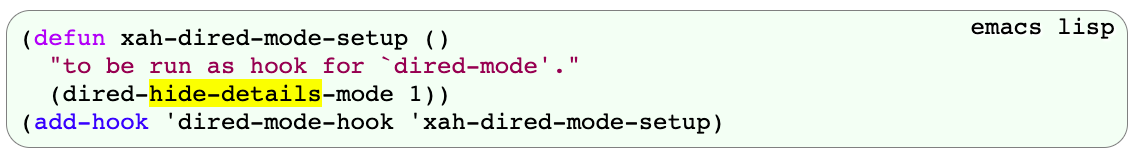
\includegraphics[width=\linewidth]{hide-details.png}

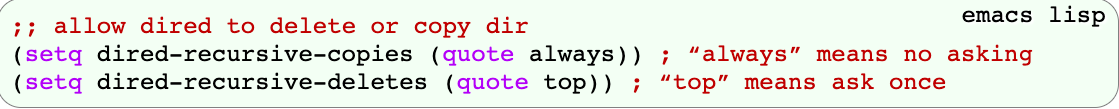
\includegraphics[width=\linewidth]{delete-directory.png}

In \underline{dired}, 
\\
Alt + x dired-do-delete [D] - delete directory
\\
\section{Copy from one dired dir to the next dired dir shown in a split window:}
\\
Put in \underline{emacs init:}
\\
\begin{verbatim} (setq dired-dwim-target t)\end{verbatim}
\\
\^\^ eval or restart emacs
\\
Now in \underline{dired}: Alt + x split-window-below, go to another dired dir
\\
When you press C to copy: the other dir in the split pane will be the default destination.
\\
Same for dired-do-rename [R], etc...
\\
Make dired use same buffer for viewing directory:
\\
In dired, Alt + x dired-find-alternate-file [a] $\Rightarrow$ open file without creating a new buffer.
\\
If you want Enter or \^ to use some buffer $\Rightarrow$ put in emacs init.
\\
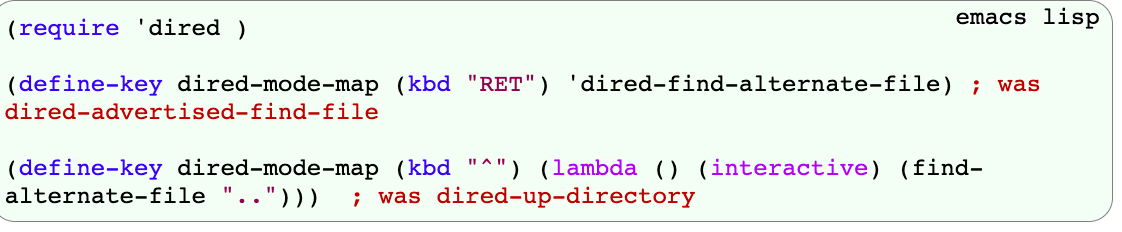
\includegraphics[width=\linewidth]{samebuffer.png}
\section{Hide Files:}
Alt + x dired-do-kill-lines [k] = hide marked files
\\
\section{Major Modes}
Always in a major mode
\section{Get a List of Major Modes:}
Alt + x apropos-command 
\\
then, type -mode
\\
Alt + x describe-variable
\\
then type auto-mode-alist
\\
What is the current major mode or how to find the value?
\\
Alt + x describe-variable
\\
then type major-mode
\\
\underline{Color Themes:}
\\
Alt + x customize-themes $\Rightarrow$ set color theme.
\\
Alt + x load-theme,
\\
then press Tab to show available themes
\\
To clear theme: Alt + x disable-theme
\\
Press Tab for Completion:
\\
\underline{To Find themes:}
\\
Alt+x describe-variable
\\
then type custom-enabled-themes
\\
set theme permissions in emacs init:
\\
(load-theme 'misterioso)
\\
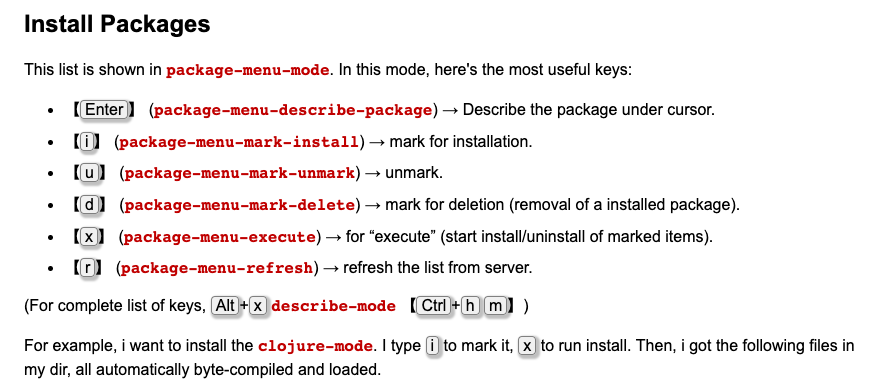
\includegraphics[width=\linewidth]{installpackages.png}
\section{Dired Navigation:}
Enter Dired for local directory:
\\
C-x d(dired)
\\
Use M-x dired to go into dired mode
\\
n/C-n/SPC = Will move down to the next line.
\\
p/C-p/Del = Will move up to the previous line.
\\
j = goto a file (dired-goto-file).
\\
M-s f C-s (dired-isearch-filenames) = forward incremental search in dired buffer.
\\
M-s f M-C-s (dired-isearch-filenames-regexp) = same as above but for reg exp.
\\
d = Flag this file for deletion (dired-flag-file-deletion).
\\
u = Remove deletion flag (dired-unmark).
\\
$<DEL>$ = Move point to previous line and remove the deletion flag on that line. (dired-unmark-backward).
\\
x = delete flags flagged for deletion (dired-do-flagged-delete).
\\
\Program{%
   \CodeComment{//Dired is on a sort of \underline{safe mode}}
   \\
   \> Try out ...
   \\
   \> dired-recursive-deletes $\rightarrow$ non-nil.
   \\
   \> delete-by-moving-to-trash $\rightarrow$ t.
}
\underline{Flagging many files at once:}
\# = Flag all auto-save files (files ending with \#) for deletion.
\\
- = Flag all backup(files with -) for deletion.
\\
. (Period) = Flag all excess numeric backup files for deletion.
\\
Oldest/newest backup files are exempt but everything in the middle is flagged.
\\
$% &$ = flag for deletion all files with certain kinds of names which suggest you could easily create those files again.
\\
$% d regexp <RET> $ = flag for deletion all files whose names match regexp.
\\
\underline{Visiting Files in Dired:}
\\
f = visit file described on current line (C-x C-f $<fileName>$) (dired-find-file).
$<RET>$
\\
e = equivalent to f.
\\
o = Like f, but creates a new window to display file-buffer (dired-find-file-other-window).
\\
v = View file described on the current line, with view mode (dired-view-fie) (read only).
\\
$^$ = Visit the parent directory of (dired-up-directory).


\end{document}

